\documentclass[12pt, letter paper]{report}
\usepackage[spanish,activeacute]{babel}
\usepackage{float}
\usepackage[letterpaper, margin = 2cm]{geometry}
\usepackage{graphicx}
\usepackage[utf8]{inputenc}

\title{
  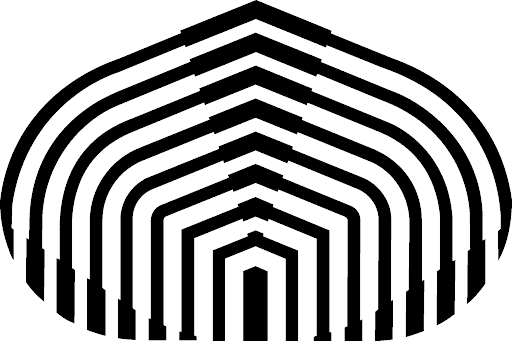
\includegraphics[height = 2cm]{images/logo.png}\\
  {\small UNIVERSIDAD SIMÓN BOLÍVAR\\
  DECANATO DE ESTUDIOS PROFESIONALES\\
  COORDINACIÓN DE INGENIERÍA DE COMPUTACIÓN}\vspace{3cm}\\
  ESTIMACIÓN DEL CONSUMO ENERGÉTICO EN BASES DE DATOS DISTRIBUIDAS\vspace{3cm}
}
\author{
  Por:\\
  Lic. Francisco Javier Márquez Hernández\vspace{1.5cm}\\
  \textbf{PROYECTO DE GRADO}\\
  Presentado ante la Ilustre Universidad Simón Bolívar\\
  como requisito parcial para optar al título de\\
  Ingeniero de Computación\\\vspace{0.5cm}
}
\date{Valle de Sartenejas, diciembre de 2025}

\renewcommand{\bibname}{Referencias}

\begin{document}
  \maketitle
  {
    \centering
    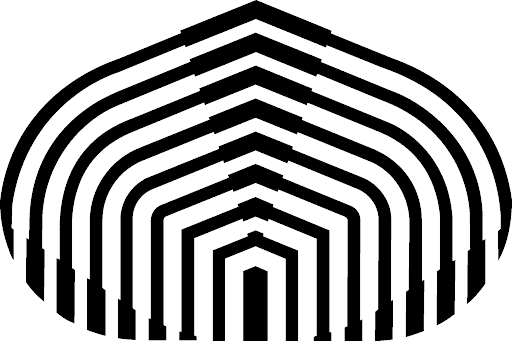
\includegraphics[height = 2cm]{images/logo.png}\\
    UNIVERSIDAD SIMÓN BOLÍVAR\\
    DECANATO DE ESTUDIOS PROFESIONALES\\
    COORDINACIÓN DE INGENIERÍA DE COMPUTACIÓN\vspace{3.5cm}\\
    \LARGE ESTIMACIÓN DEL CONSUMO ENERGÉTICO EN BASES DE DATOS DISTRIBUIDAS
    \vspace{3.5cm}
  
    \large Por:\\
    Lic. Francisco Javier Márquez Hernández\vspace{1.7cm}\\
    Realizado con la asesoría de:\\
    Dr. Marlene Goncalves Da Silva\vspace{1.7cm}\\
    \textbf{PROYECTO DE GRADO}\\
    Presentado ante la Ilustre Universidad Simón Bolívar\\
    como requisito parcial para optar al título de\\
    Ingeniero de Computación\\\vspace{1.7cm}
  
    Valle de Sartenejas, diciembre de 2025
  
    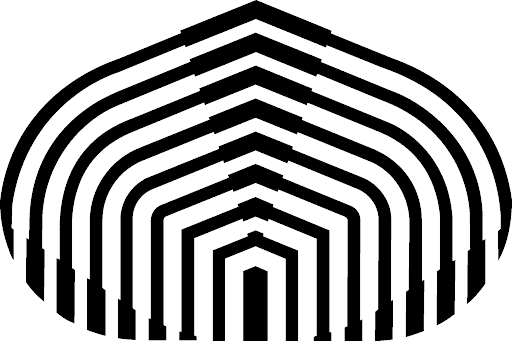
\includegraphics[height = 2cm]{images/logo.png}\\
    UNIVERSIDAD SIMÓN BOLÍVAR\\
    DECANATO DE ESTUDIOS PROFESIONALES\\
    COORDINACIÓN DE INGENIERÍA DE COMPUTACIÓN\vspace{3.5cm}\\
    \LARGE ESTIMACIÓN DEL CONSUMO ENERGÉTICO EN BASES DE DATOS DISTRIBUIDAS
    \vspace{3.5cm}
  
    \large Por:\\
    Lic. Francisco Javier Márquez Hernández\vspace{1.7cm}\\
    Realizado con la asesoría de:\\
    Dr. Marlene Goncalves Da Silva\vspace{1.7cm}\\
    \textbf{RESUMEN}\\
  }
  Aquí va el resumen, máximo trescientas (300) palabras. Se elabora al final de
  todo el libro. Lleva palabras clave al final.

  \textbf{Palabras clave}: Palabra 1, Palabra 2, Palabra 3, Palabra 4, Palabra
  5.
  \newpage
  \addcontentsline{toc}{chapter}{\textbf{DEDICATORIA}}
  \begin{center}
    \large \textbf{DEDICATORIA}
  \end{center}

  Dedico esto a...

  \newpage
  \addcontentsline{toc}{chapter}{\textbf{AGRADECIMIENTOS}}
  \begin{center}
    \Large \textbf{AGRADECIMIENTOS}
  \end{center}

  Agradezco a...

  \tableofcontents
  \addcontentsline{toc}{chapter}{\textbf{Índice general}}

  \newpage
  \addcontentsline{toc}{chapter}{\textbf{Introducción}}
  \begin{center}
    \Large \textbf{Introducción}
  \end{center}

  \chapter{I. Planteamiento del problema} % (fold)
  \label{cha:i_planteamiento_del_problema}
    \section{Planteamiento del problema} % (fold)
    \label{sec:planteamiento_del_problema}
        El consumo energético de los sistemas humanos y la generación de
        alternativas más eficientes ha sido un interés para el mundo desde la
        segunda mitad del siglo XX, cuando aparece la primera gran alerta sobre
        este particular y en el siglo XXI se formaliza este interés en los
        procesos informáticos. En el particular de los procesos informáticos, el
        auge que se ha visto con el crecimiento acelarado del internet y la
        migración de los sistemas analógicos y físicos hacia sistemas virtuales
        orientó el interés del consumo energético y la eficiencia hacia los
        manejadores de bases de datos, que son la columna vertebral de muchos
        sistemas.

        El estudio de la eficiencia de las consultas y su consumo energético no
        ha estado presente desde el comienzo, aunque su enfoque ha sido más
        limitado hacia la eficiencia de las consultas sobre sistemas de bases de
        datos centralizadas. En los últimos años, se han empezado estudios sobre
        los sistemas de bases de datos distribuidas. Sin embargo, estos estudios
        aún requieren mucha más atención a los múltiples factores que afectan la
        eficiencia de las consultas y el consumo energético asociado a cada una.

        Es por este motivo que se presenta una aproximación al estudio del
        consumo energético y la eficiencia de las consultas de manejadores de
        bases de datos relacionales PostgreSQL y MySQL (distribuidas) a los
        efectos de ampliar la compresión sobre los posibles cuellos de botella
        que incrementan el uso de recursos de un computador y por tanto, el
        consumo energético.
    % section planteamiento_del_problema (end)

    \section{Objetivos} % (fold)
    \label{sec:objetivos}
      \subsection{Objetivo general} % (fold)
      \label{sub:objetivo_general}
        Comparar el rendimiento y el consumo energético en un ambiente
        distribuido, con y sin diseño físico, mediante las pruebas de
        rendimiento TPC-H y los sistemas de bases de datos PostgreSQL y MySQL.
      % subsection objetivo_general (end)

      \subsection{Objetivos específicos} % (fold)
      \label{sub:objetivos_específicos}
        \begin{enumerate}
          \item Preparar el entorno y los datos de prueba con las pruebas de
          rendimiento TPC-H.
          \item Configurar un clúster con los sistemas de bases de datos.
          \item Analizar los resultados de las pruebas mediante...
        \end{enumerate}
      % subsection objetivos_específicos (end)
    % section objetivos (end)
  % chapter i_planteamiento_del_problema (end)

  \chapter{II. Marco teórico} % (fold)
  \label{cha:ii_marco_teórico}
    \section{Antecedentes} % (fold)
    \label{sec:antecedentes}
      Antecedentes
    % section antecedentes (end)
    \section{Bases teóricas} % (fold)
    \label{sec:bases_teóricas}
      Bases teóricas
    % section bases_teóricas (end)
  % chapter ii_marco_teórico (end)

  \chapter{III. Marco metodológico} % (fold)
  \label{cha:iii_marco_metodológico}
    \section{Equipos} % (fold)
    \label{sec:equipos}
      Equipos, hardware, específicaciones
    % section equipos (end)

    \section{Metodología experimental} % (fold)
    \label{sec:metodología_experimental}
      Metodología experimental
    % section metodología_experimental (end)
  % chapter iii_marco_metodológico (end)

  \chapter{IV. Resultados y discusión} % (fold)
  \label{cha:iv_resultados_y_discusión}
    Aquí van los resultados con su respectiva discusión
  % chapter iv_resultados_y_discusión (end)

  \newpage
  \addcontentsline{toc}{chapter}{\textbf{Conclusión}}
  \begin{center}
    \Large \textbf{Conclusión}
  \end{center}

  \addcontentsline{toc}{chapter}{\textbf{Referencias}}
  \bibliographystyle{apalike}
  \bibliography{Refs} %Cambiar el título
  \nocite{*}
\end{document}
